
\begin{figure}
\begin{center}
    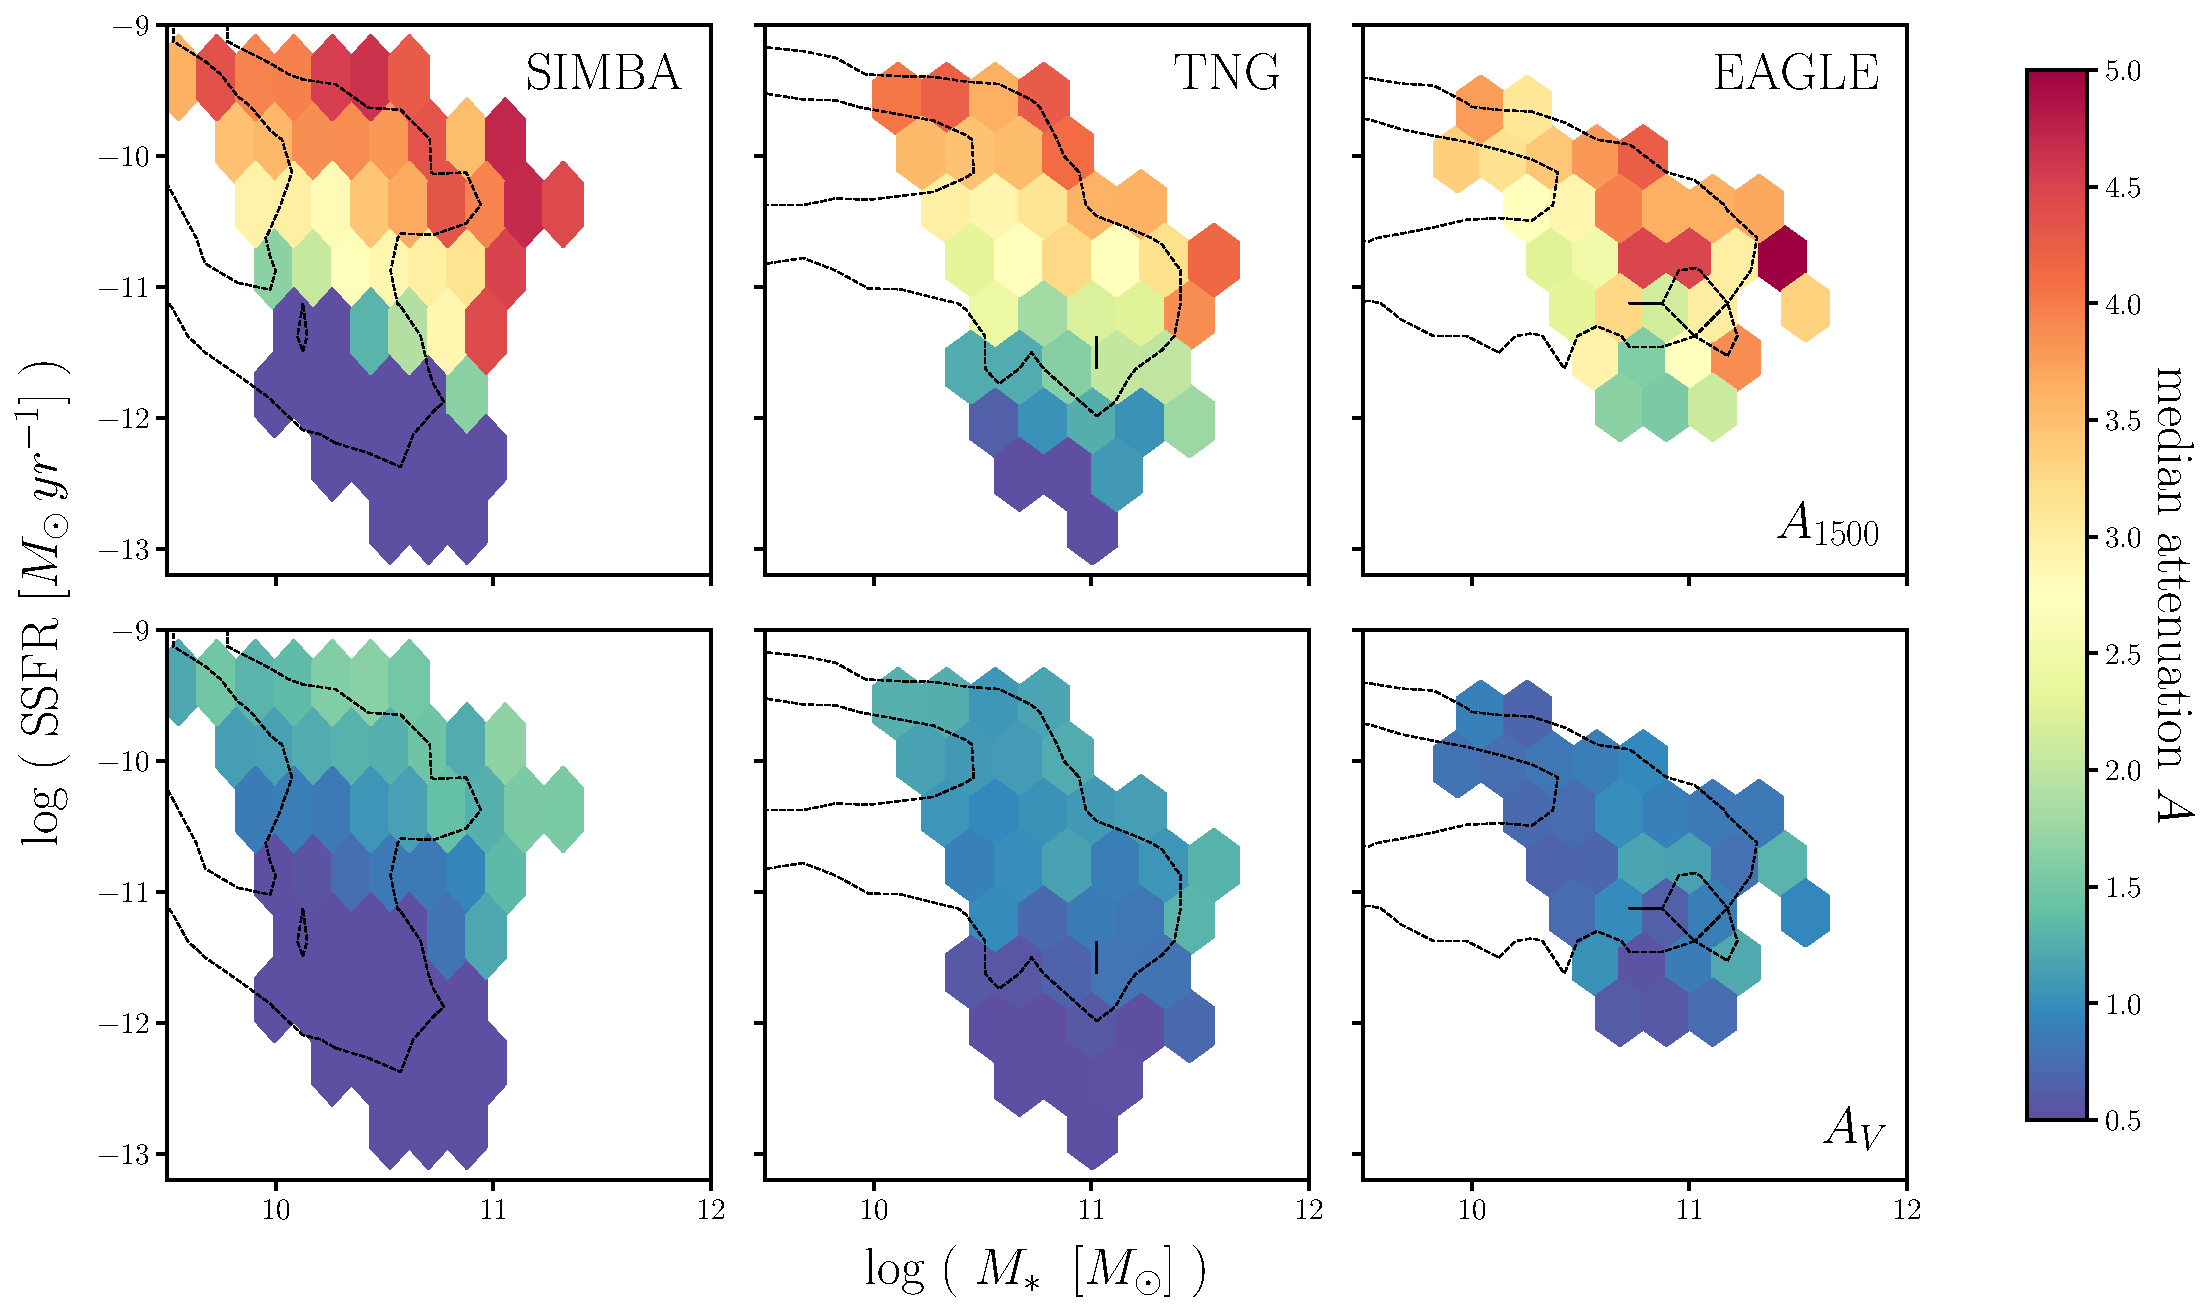
\includegraphics[width=0.9\textwidth]{figs/abc_av_mssfr.pdf}
    \caption{\label{fig:avmsfr}
    \chedit{ 
        $M_*$ and $\ssfr$ dependence of dust attenuation at $1500 \AA$, $A_{1500}$,
        and at $5500\AA$, $A_{V}$.
    }
    }
\end{center}
\end{figure}

\subsection{The Galaxy -- Dust Connection}  
\chedit{
    With the \eda~framework, we can also shed light on the connection between
    the physical properties of galaxies and dust attenuations.
    In our \eda~prescription, we included a flexible $M_*$ and $\ssfr$ dependence in both the
    amplitude and slope of the attenuation curve~(Eqs~\ref{eq:tauv}
    and~\ref{eq:delta}. 
    Hence, we can reveal the $M_*$ and $\ssfr$ dependence of dust attenuation
    through the \eda~parameter constraints (Figure~\ref{fig:abc}) and the
    predicted attenuation curves. 
}


\chedit{
    Focusing first on the amplitude of dust attenuation, we find that TNG has
    little $M_*$ dependence in $\tau_V$: 
    $\mtaum = 0.14\substack{+0.64 \\ -0.58}$. 
    EAGLE has a more significant positive $M_*$ dependence:
    $\mtaum = 0.53\substack{+0.36 \\ -0.36}$.
    Though neither TNG nor EAGLE has a strong dependence, $V$-band dust
    attenuation is higher for more massive galaxies.  
    Meanwhile, we find significant $\ssfr$ dependences in both TNG 
    ($\mtaus = -0.42\substack{+0.2 \\ -0.18}$)
    and EAGLE
    ($\mtaus = -0.24\substack{+0.22 \\ -0.19}$): galaxies with higher $\ssfr$
    have lower $V$-band dust attenuation. 
    For the slope of the dust attenuation, we find significant $M_*$
    dependence in both TNG 
    ($\mdeltam = -0.36\substack{+0.23\\-0.19}$)
    and EAGLE
    ($\mdeltam = -0.2\substack{+0.16\\-0.16}$). 
    More massive galaxies have steeper attenuation curves. 
    We also find strong $\ssfr$ dependence in both TNG 
    ($\mdeltas = -0.55\substack{+0.08 \\ -0.08}$)
    and EAGLE
    ($\mdeltas = -0.43\substack{+0.08 \\ -0.08}$).
    Galaxies with higher $\ssfr$ have steeper attenuation curves.

}

\chedit{
    Next, we take a closer look at the $M_*$ and $\ssfr$ dependence of the
    attenuation curve in Figure~\ref{fig:avmsfr}. We present dust attenuation
    at $1500\AA$ ($A_{1500}$; top) and $5500\AA$ ($A_V$; bottom) as a function
    of $\log M_*$ and $\log {\rm SFR}$ predicted by the \eda~for TNG (left) and
    EAGLE (right). For each hexagonal bin, the colormap represents the median
    attenuation for all simulated galaxies in the bin. We only include
    $A_{1500}$ or $A_V$ values for galaxies that satisfy our $M_r < -20$
    completeness limit. The bottom panels of Figure~\ref{fig:avmsfr}
    corroborate our conclusions on $V$-band dust attenuation from the
    \eda~parameter posteriors (Figure~\ref{fig:abc}): $A_V$ has a slight $M_*$
    dependence but a significant $\ssfr$ dependence. 
    Furthermore, by comparing the top to the bottom panels, we can confirm the
    $M_*$ and $\ssfr$ dependence of the  attenuation curve slopes. 
}


The $M_*$ dependence in $\tau_V$ and $\delta$
are further illustrated in the attenuation curves in Figure~\ref{fig:raw_atten}.
For TNG, there is little difference in the $V$-band attenuation between the 
top and bottom panels. However, more massive galaxies have steeper slopes 
with similar $A_V$ so they have significantly higher UV attenuation. For
EAGLE, more massive galaxies have both higher $V$-band and UV attenuation.
Overall, we find that more massive galaxies have higher attenuation,
which is consistent with the literature. \cite{burgarella2005}, for instance,
found significant positive $M_*$ dependence in $FUV$ attenuation in
NUV-selected and FIR-selected samples. \cite{garn2010} and \cite{battisti2016}
also find higher attenuation in more massive SDSS star-forming galaxies. Most
recently, \cite{salim2018} find higher $V$ and $FUV$ attenuation for more
masssive star-forming galaxies in GSWLC2. 

From the attenuation curves in
Figure~\ref{fig:raw_atten}, we similarly find that star-forming galaxies have
attenuation curves with slightly lower $A_V$ but substantially higher UV 
attenuation. Quiescent galaxies, on the other hand, have significantly 
shallower attenuation curves. Although observations have examined the
SSFR dependence of dust attenuation, they cannot be compared to our findings since
they focus only on star-forming galaxies, due to the difficulty in
observationally constraining the attenuation curve in quiescent
galaxies~\citep[\eg][]{garn2010, reddy2015, battisti2016, battisti2017, salim2018}. 
In summary, from the bestfit \eda~models of TNG and EAGLE, we find that
\emph{galaxies with higher $M_*$ have overall higher dust attenuation and
galaxies with higher SSFR have steeper attenuation curves}.
